\atsptt
\begin{frame}{\ft{Coordinated Data Visualization}}
\section{Group 1: Coordinated Data Visualization}

	\pdfpageheight 30cm
	
\begin{annotatedFigure}{2mm}{-1mm}{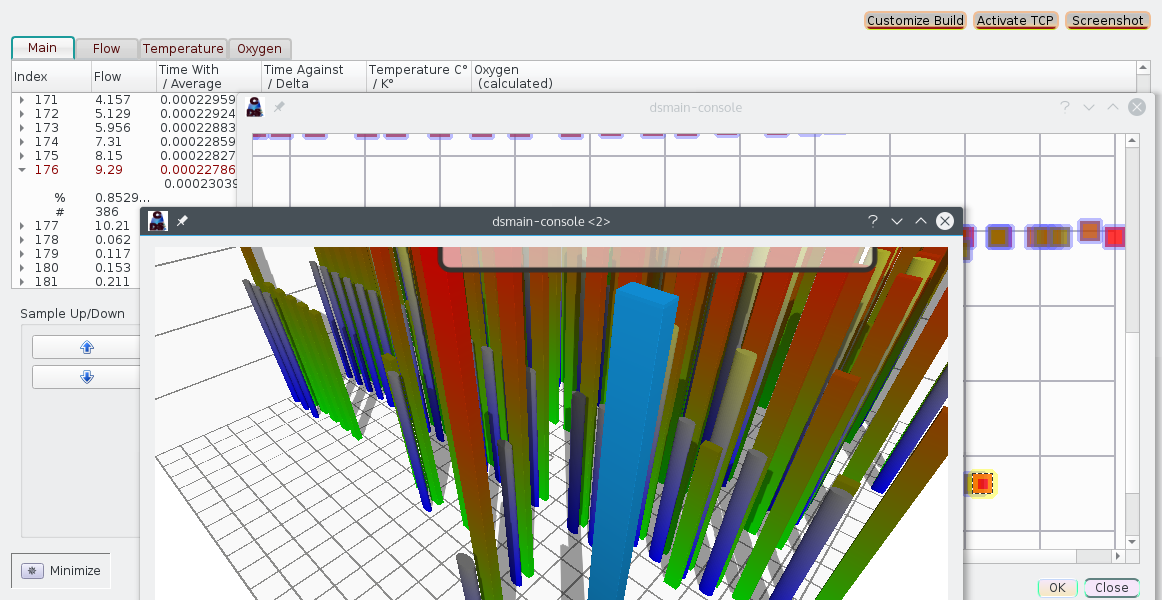
\includegraphics[scale=1]{texs/coord.png}}
  \node [anchor=west,inner sep=14, text width=8.7cm,
  line width=1mm, fill opacity=0.9,
  draw = blue!20!black,
  top color=white,text=black,
  bottom color=blue!40,
  rounded corners=6pt
  %blur shadow={shadow blur steps=2}
  ]
  at (0.67,0.72){\annfont\textbf{Dataset Applications can use 2D and 3D 
  		visualization as well as textual/tabular displays, employing Reactive 
  		Programming techniques to coordinate multiple visible windows.  For example, 
  		visual cues direct attention to selected samples represented via 
  		expanded rows (\circled{1}), color-highlighted 2D regions (\circled{2}), 
  		and color-highlighted 3D bars (\circled{3}).  The main window and 2D and 3D windows are functionally linked so that the same sample is 
  		highlighted/expanded in each display window.}};
  
              \annotatedFigureBox{0.02,0.63}{0.057,0.74}{1}{0.057,0.74}%
              \annotatedFigureBox{0.825,0.16}{0.86,0.23}{2}{0.856,0.24}%            
              \annotatedFigureBox{0.55,0.42}{0.55,0.48}{3}{0.55,0.48}     
              
\end{annotatedFigure}	
%\end{figure}
\end{frame}

